\documentclass[xcolor=dvipsnames]{beamer}

\usepackage[font=scriptsize,labelfont=bf]{caption}
\usepackage{url}
\usepackage{hyperref}
\usepackage{verb atim}
\usepackage{amsmath}
\usepackage{graphicx}
\usepackage{ragged2e}
\usepackage{tcolorbox}
\usepackage[dvipsnames]{xcolor}
\usepackage{ulem}
\usepackage{adjustbox}
\usepackage{subcaption}
\usepackage{dirtytalk}
\usepackage{xcolor}
\usepackage{listings}
\usepackage{mathtools}

% Definir colores
\definecolor{codegreen}{rgb}{0,0.6,0}
\definecolor{codegray}{rgb}{0.5,0.5,0.5}
\definecolor{codeblue}{rgb}{0,0,1}
\definecolor{backcolour}{rgb}{0.95,0.95,0.92}
\definecolor{crimson}{rgb}{0.86, 0.08, 0.24}
\definecolor{UBCblue}{rgb}{0.04706, 0.13725, 0.26667} % UBC Blue (primary)
\definecolor{UBCgrey}{rgb}{0.3686, 0.5255, 0.6235} % UBC Grey (secondary)

% Configuración de lstlisting
\lstdefinestyle{mystyle}{
    backgroundcolor=\color{backcolour},   
    commentstyle=\color{codegreen},
    keywordstyle=\color{codeblue}\bfseries,
    numberstyle=\tiny\color{codegray},
    stringstyle=\color{red},
    basicstyle=\ttfamily\footnotesize,
    breakatwhitespace=false,         
    breaklines=true,                 
    captionpos=b,                    
    keepspaces=true,                 
    % numbers=left,                    
    numbersep=5pt,                  
    showspaces=false,                
    showstringspaces=false,
    showtabs=false,                  
    tabsize=2,
    literate={-}{{-}}1 {~}{{\textasciitilde}}1  % Corrige guiones y tildes
}
\lstset{style=mystyle}

\usetheme{Madrid}
%\useoutertheme[subsection=false]{smoothbars}

\AtBeginSection[]{
  \begin{frame}
  \vfill
  \centering
  \begin{beamercolorbox}[sep=8pt,center,shadow=true,rounded=true]{title}
    \usebeamerfont{title}\secname\par%
  \end{beamercolorbox}
  \vfill
  \end{frame}
}

\DeclareMathOperator*{\concat}{\mathbin\Vert}

\setbeamercolor{palette primary}{bg=UBCblue,fg=white}
\setbeamercolor{palette secondary}{bg=UBCblue,fg=white}
\setbeamercolor{palette tertiary}{bg=UBCblue,fg=white}
\setbeamercolor{palette quaternary}{bg=UBCblue,fg=white}
\setbeamercolor{structure}{fg=UBCblue} % itemize, enumerate, etc
\setbeamercolor{section in toc}{fg=UBCblue} % TOC sections

\renewcommand{\figurename}{Fig.}
%\logo{\includegraphics[height=1.2cm]{img/logo_di_black.png}}

% Override palette coloring with secondary
\setbeamercolor{subsection in head/foot}{bg=UBCgrey,fg=white}

\setbeamertemplate{navigation symbols}{} %Deactivate the interactive buttons

\title[Introducción a Modelos Supervisados - T3]{Introducción a Modelos Supervisados}
\date{2025-04-11}
\author[CNF]{Camilo Esteban Núñez Fernández}
\institute[DI UTFSM]{INF396 - Introducción a la Ciencia de Datos\\ Departamento de Informática}

\begin{document}
	\begingroup 
        \setbeamertemplate{headline}{}
        \begin{frame}
            \titlepage
        \end{frame}
    \endgroup

    \section{Definición de \textit{Aprendizaje}}
    \begin{frame}{I~$\rhd$~Sobre IA, ML, y DL}
        \begin{figure}
            \centering
            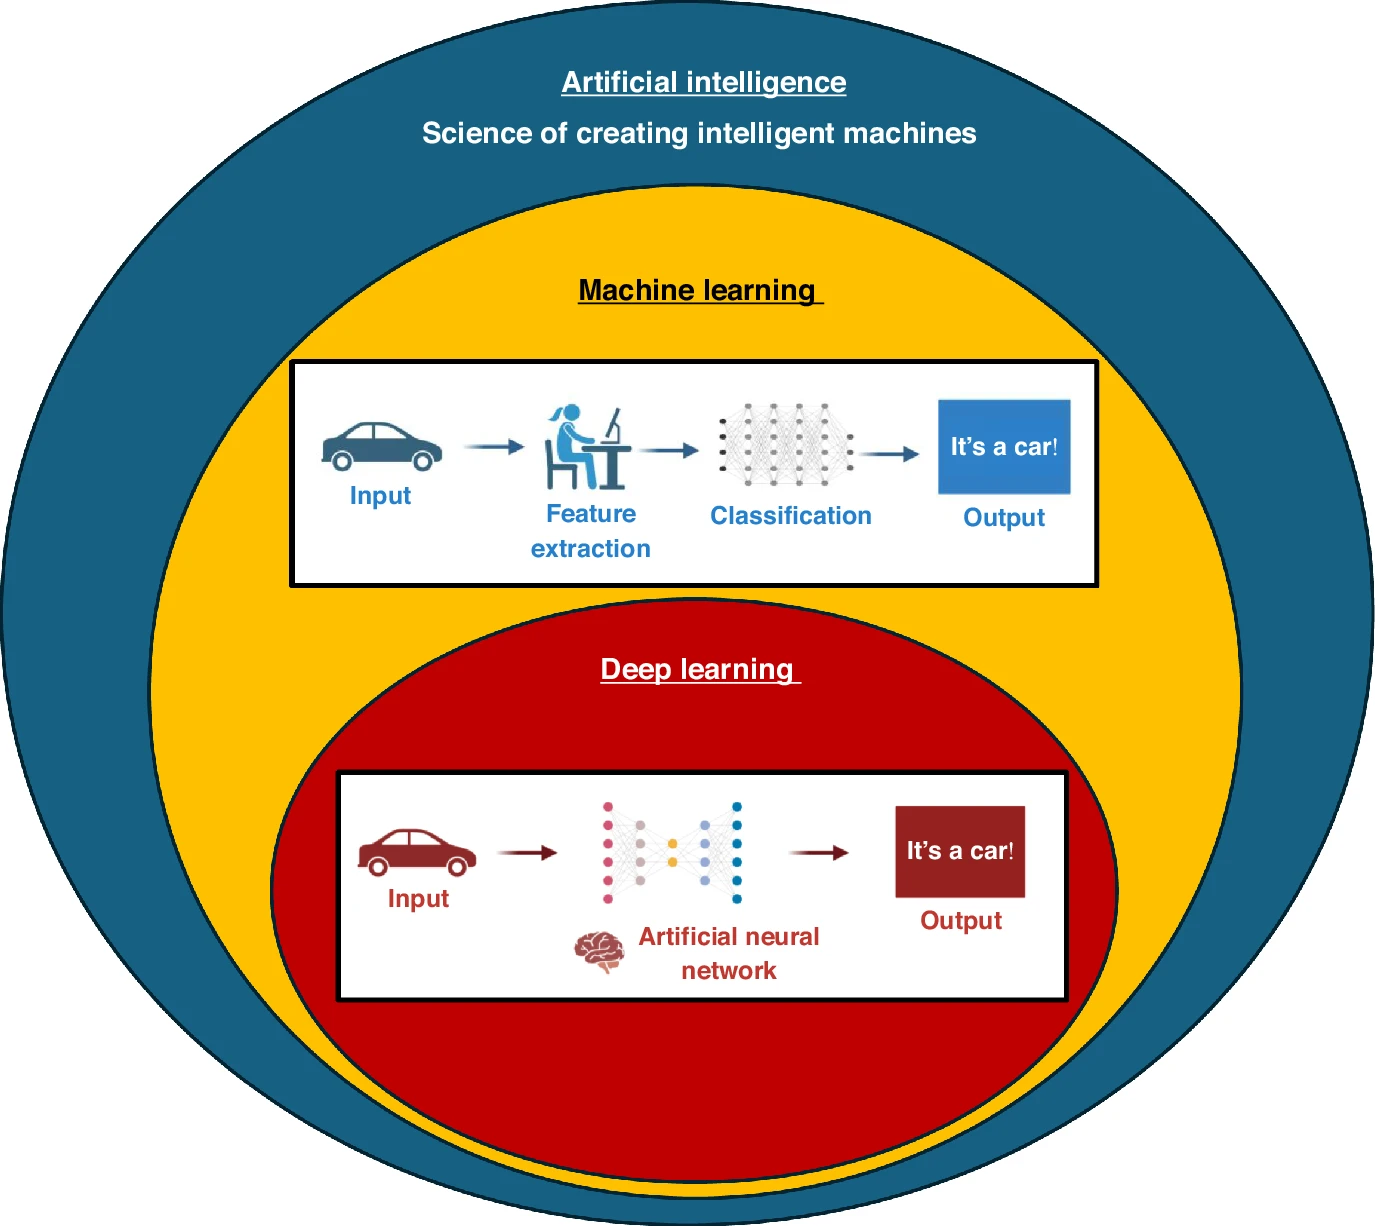
\includegraphics[width=0.6\linewidth]{imgs/sec1/s44276-025-00135-4-img1.png}
            \caption{Diagrama de Venn para relaciones entre AI, ML y DL.\footnote{\tiny{O’Connor, O., McVeigh, T.P. Increasing use of artificial intelligence in genomic medicine for cancer care- the promise and potential pitfalls. BJC Rep 3, 20 (2025). \url{https://doi.org/10.1038/s44276-025-00135-4}}}}
        \end{figure}
    \end{frame}

    \begin{frame}{I~$\rhd$~Definición de \textit{Aprendizaje}}
    \begin{columns}
        \column{0.3\textwidth}
            \textbf{Tom Michael Mitchell}
            \begin{figure}
            \centering
            
\includegraphics[width=0.6\textwidth]{imgs/sec1/213030.jpg}
            \end{figure}
            \textit{\scriptsize{Machine Learning, Mitchell, T.M., 1997, McGraw-Hill Education.}}
        \column{0.65\textwidth}
            %\pause
            \begin{block}{Definición}
            A computer program is said to \textbf{learn} from experience \( E \) with respect to some class of tasks \( T \) and performance measure \( P \), if its performance at tasks in \( T \), as measured by \( P \), improves with experience \( E \).
            \end{block}
    \end{columns}    
    \end{frame}

    \begin{frame}{I~$\rhd$~Definición de \textit{Aprendizaje}}
    \framesubtitle{Ejemplo: Handwritten Digits Classification}
       \begin{columns}
        \column{0.65\textwidth}
            \textbf{Clasificación de Dígitos Escritos a Mano}
            \begin{itemize}
                \item \textit{Task \( T \)}: Reconocer y clasificar dígitos escritos a mano desde una imagen.
                \item \textit{Performance Measure \( P \)}: Porcentaje de dígitos clasificados correctamente.
                \item \textit{Training Experience \( E \)}: Secuencia de imágenes etiquetas con dígitos.
            \end{itemize}
        \column{0.3\textwidth}
            \begin{figure}
                \centering
                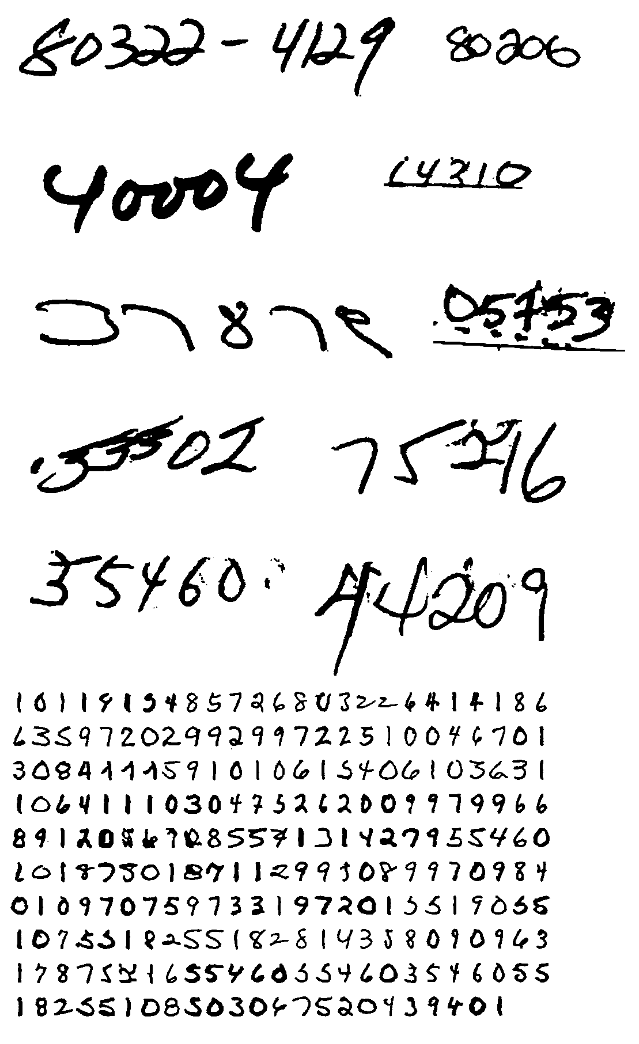
\includegraphics[width=\linewidth]{imgs/sec1/0899-7667-img1.png}
            \end{figure}
        \end{columns} 
    \end{frame}

    \begin{frame}{I~$\rhd$~Definición de \textit{Aprendizaje}}
    \framesubtitle{Ejemplo: Handwritten Digits Classification}
       \begin{figure}
           \centering
           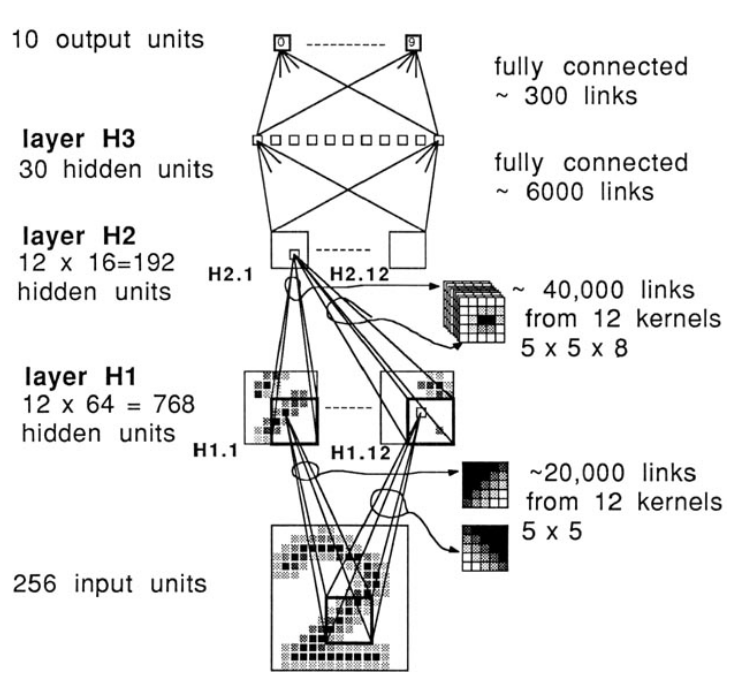
\includegraphics[width=0.5\linewidth]{imgs/sec1/0899-7667-img2.png}
           \caption{\scriptsize{Y. LeCun, B. Boser, J. S. Denker, D. Henderson, R. E. Howard, W. Hubbard, L. D. Jackel; Backpropagation Applied to Handwritten Zip Code Recognition. Neural Comput 1989; 1 (4): 541–551. doi: \url{https://doi.org/10.1162/neco.1989.1.4.541}}}
       \end{figure}
    \end{frame}

    \section{Definición \textit{Task} \( T \)}
    \begin{frame}{II~$\rhd$~Definición de \textit{Aprendizaje}}
    \framesubtitle{Definición \textit{Task} \( T \)}
        \begin{block}{Definición \textit{Task} \( T \)}
        Es el \textbf{problema} que busca resolver nuestro programa.
        \end{block}
        \vspace{5mm}
        %\pause
        \begin{itemize}
            \item Ejemplos:
            \begin{itemize}
                \item Clasificar imagen de un dibujo.
                \item Detectar la figura de los autos en una imagen.
                \item Clasificar una anomalía en una serie de tiempo.
                \item Generar la descripción de una imagen.
            \end{itemize}
        \end{itemize}
    \end{frame}

    \begin{frame}{II~$\rhd$~Definición de \textit{Aprendizaje}}
    \framesubtitle{Definición \textit{Task} \( T \)}
        \begin{block}{Definición}
        La \textit{Task} \( T \) se puede formalizar como una función o transformación $f^{*}$ tal que: $f^{*}:\mathcal{X}~\rightarrow~\mathcal{Y}$.
        \end{block}
        %\pause
        \vspace{5mm}
        \begin{figure}
            \centering
            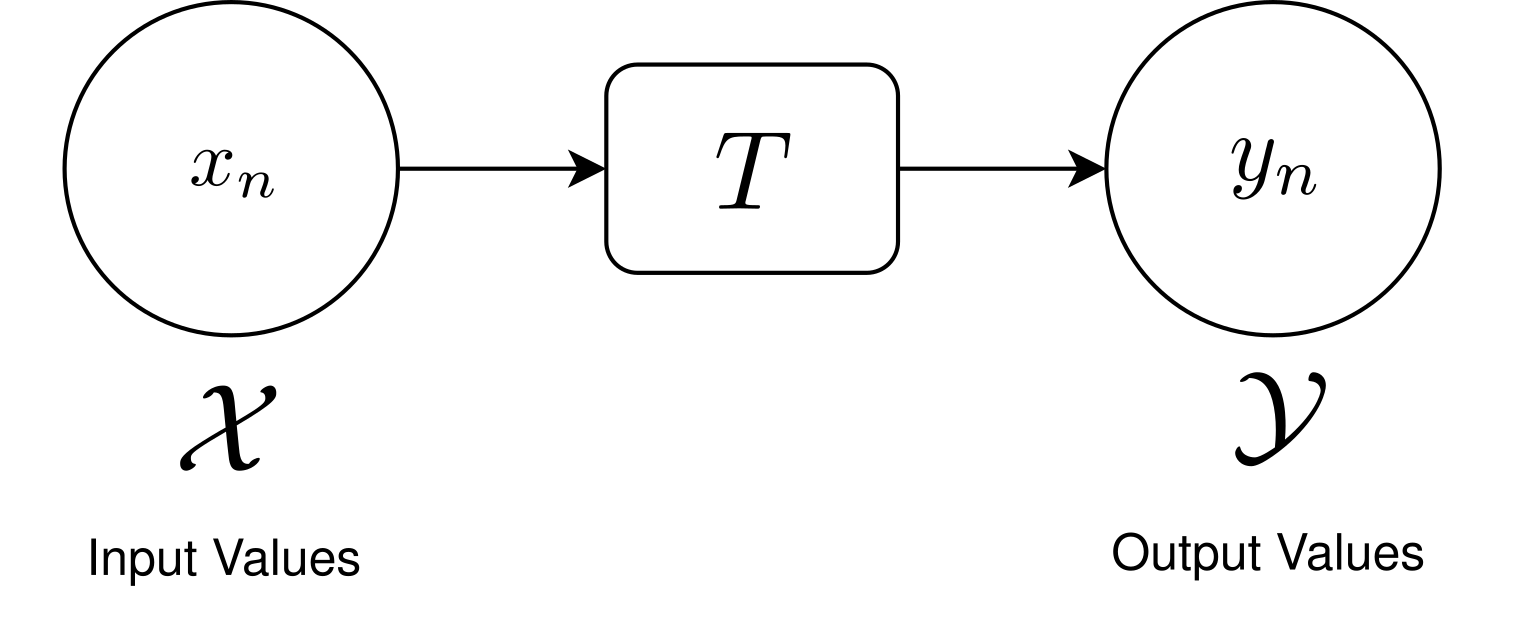
\includegraphics[width=0.8\linewidth]{imgs/def01/task01.png}
        \end{figure}
    \end{frame}

    \begin{frame}{II~$\rhd$~Definición de \textit{Aprendizaje}}
    \framesubtitle{Definición \textit{Task} \( T \)}
        \begin{block}{Definición}
        La $f^{*}$ es \textbf{desconocida}, sólo sabes qué elementos toma en un \textbf{dominio}~$\mathcal{X}$ y qué elementos toma en el \textbf{codominio}~$\mathcal{Y}$.
        \end{block}
        %\pause
        \vspace{5mm}
        \begin{figure}
            \centering
            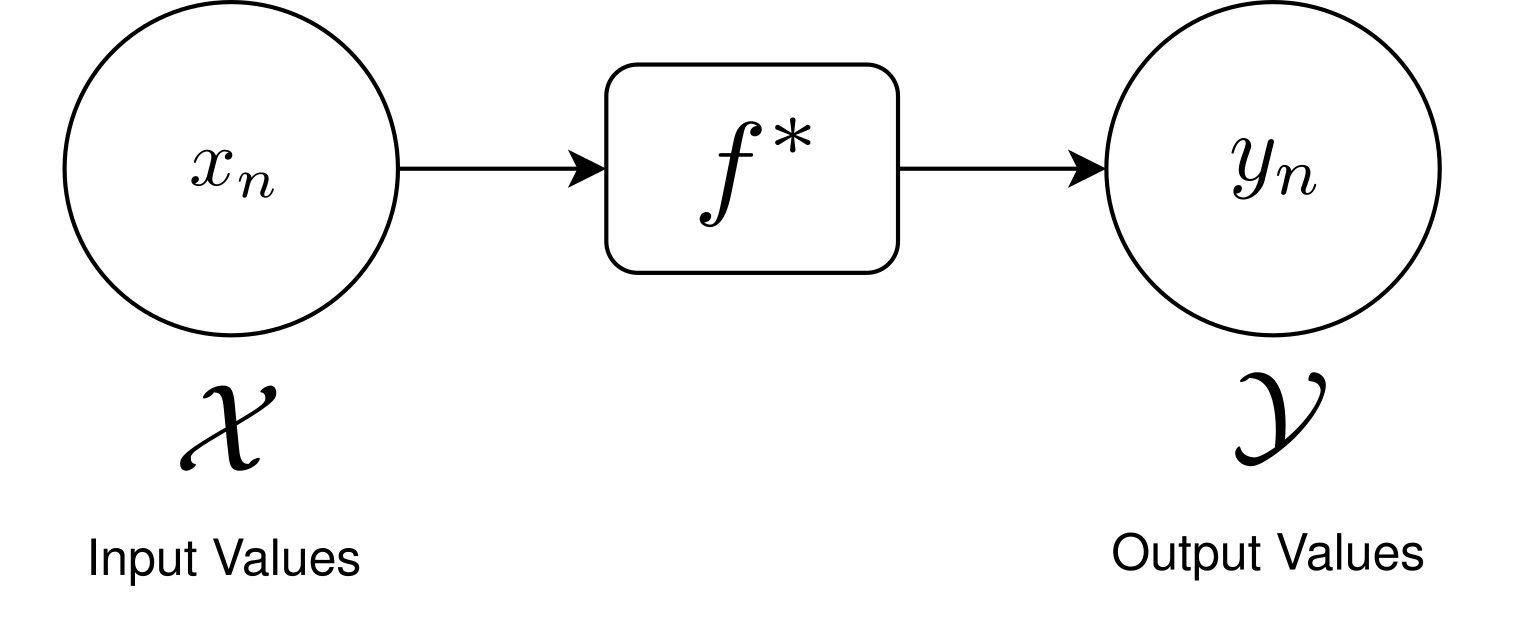
\includegraphics[width=0.8\linewidth]{imgs/def01/task02.png}
        \end{figure}
        %\pause
        \textcolor{DarkOrchid}{Buscamos aproximar $f^{*}$ según nuestros datos !}
    \end{frame}

    \begin{frame}{II~$\rhd$~Definición de \textit{Aprendizaje}}
    \framesubtitle{Tipos de \textit{Task} \( T \)}
        \textbf{\Large{\( T \): Clasificación}}
        \vspace{2mm}
        \begin{itemize}
            \item \textcolor{crimson}{Problema} que busca predecir aquellos valores \textcolor{crimson}{cualitativos o categóricos} del espacio $\mathcal{Y}$.
            \vspace{1mm}
            \begin{figure}
                \centering
                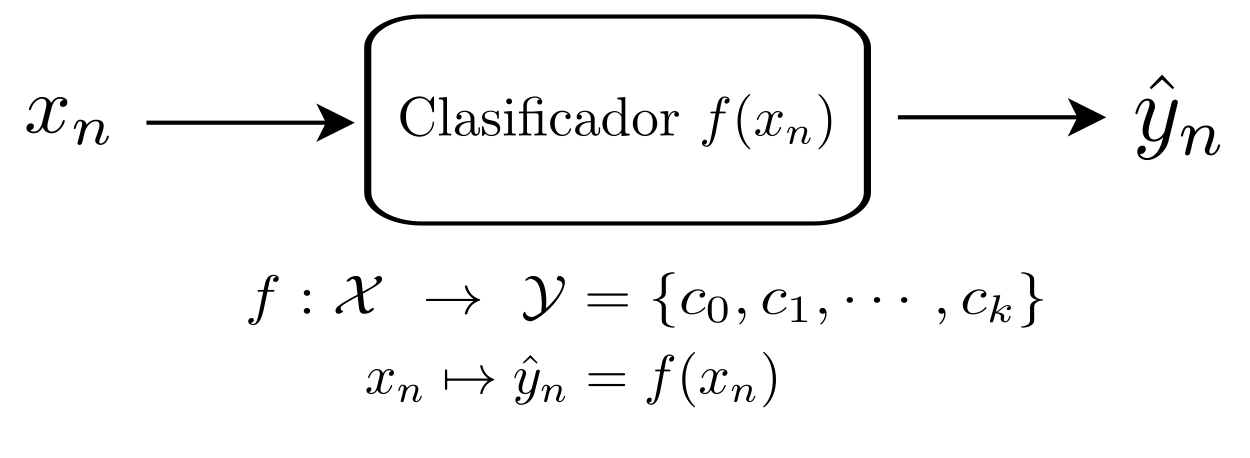
\includegraphics[width=0.9\linewidth]{imgs/def01/task03.png}
            \end{figure}
        \end{itemize}
    \end{frame}

    \begin{frame}{II~$\rhd$~Definición de \textit{Aprendizaje}}
    \framesubtitle{Tipos de \textit{Task} \(T\)}
        \textbf{\Large{\( T \): Clasificación}}
        \begin{figure}
            \centering
            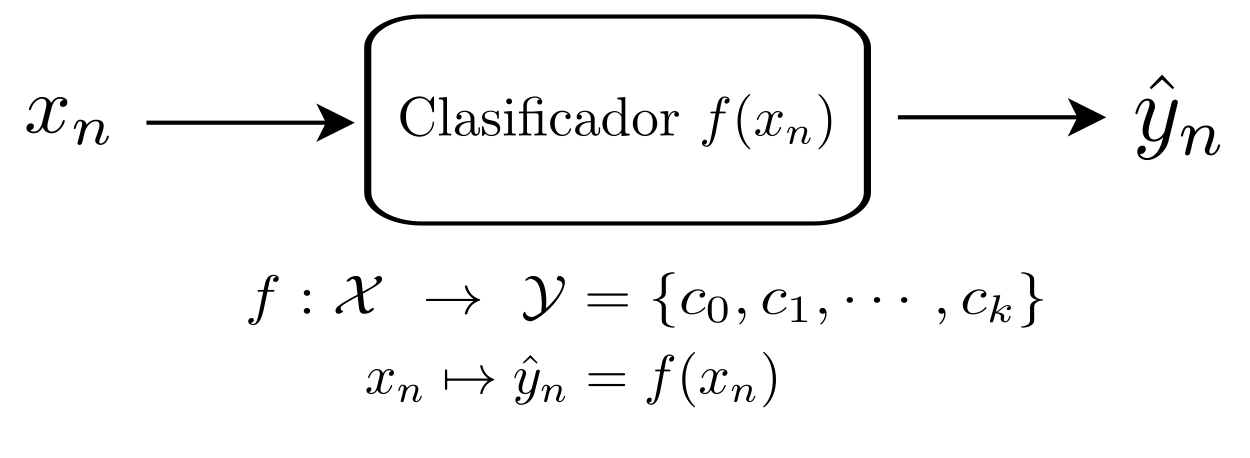
\includegraphics[width=0.55\linewidth]{imgs/def01/task03.png}
        \end{figure}
        \begin{itemize}
            %\pause
            \item Por definición canónica (o histórica), de la ecuación $\hat{y}_{n}=f(x_{n})$, desprenderemos el termino $f(x_{n})$, y lo llamaremos la \textbf{\textcolor{crimson}{hipotiposis}}.\footnote{\scriptsize{Es normal encontrar textos donde se sobrescribe $f^{*}:\mathcal{X}~\rightarrow~\mathcal{Y}$, como $h:\mathcal{X}~\rightarrow~\mathcal{Y}$, y donde $h$ es la \textbf{hipótesis} y a su vez de función que busca predecir el valor de $y_{n}$.}}
            %\pause
            \item En este caso, $x_{n}$, \textbf{SOLO} puede ser asignado a \textbf{UN} elemento (o categoría) $c$. Las categorías $c$ son mutuamente excluyentes, no se pueden dar simultáneamente.
        \end{itemize}
    \end{frame}

    \begin{frame}{II~$\rhd$~Definición de \textit{Aprendizaje}}
    \framesubtitle{Tipos de \textit{Task} \( T \)}
        \textbf{\Large{\( T \): Clasificación Multi-Label}}
        \vspace{2mm}
        \begin{itemize}
            \item \textcolor{crimson}{Problema} que busca predecir aquellos valores \textcolor{crimson}{\textbf{múltiples} cualitativos o categóricos} del espacio $\mathcal{Y}$.
            \vspace{1mm}
            \begin{figure}
                \centering
                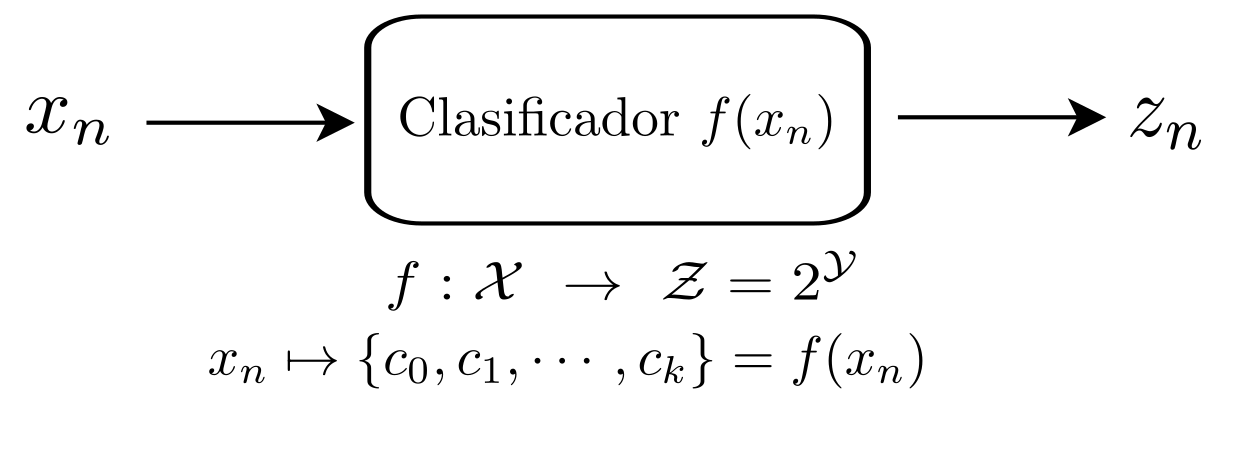
\includegraphics[width=0.9\linewidth]{imgs/def01/task04.png}
            \end{figure}
        \end{itemize}
    \end{frame}

    \begin{frame}{II~$\rhd$~Definición de \textit{Aprendizaje}}
    \framesubtitle{Tipos de \textit{Task} \(T\)}
        \textbf{\Large{\( T \): Clasificación Multi-Label}}
        \begin{figure}
            \centering
            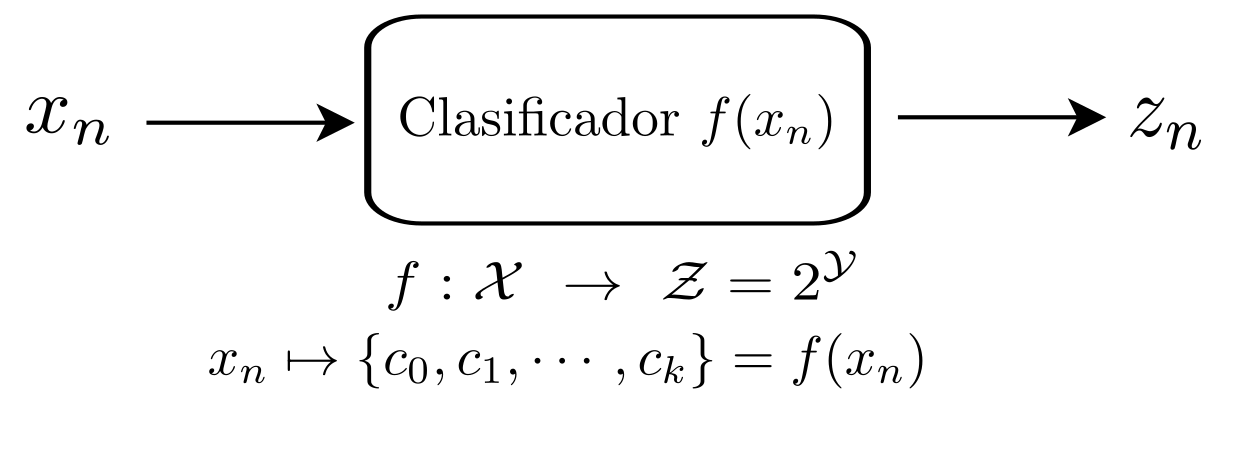
\includegraphics[width=0.55\linewidth]{imgs/def01/task04.png}
        \end{figure}
        \begin{itemize}
            \item En este caso, $x_{n}$, puede ser asignado a \textbf{UNA o MÁS} categorías $c$. Las categorías $c$ \textcolor{crimson}{no son} mutuamente excluyentes, y \textcolor{crimson}{sí pueden dar simultáneamente}.
        \end{itemize}
    \end{frame}

    \begin{frame}{II~$\rhd$~Definición de \textit{Aprendizaje}}
    \framesubtitle{Tipos de \textit{Task} \( T \)}
        \textbf{\Large{\( T \): Regresión}}
        \vspace{2mm}
        \begin{itemize}
            \item \textcolor{crimson}{Problema} que busca predecir aquellos valores \textcolor{crimson}{cuantitativos o continuos en $\Re$} del espacio $\mathcal{Y}\subset\Re$.
            \vspace{1mm}
            \begin{figure}
                \centering
                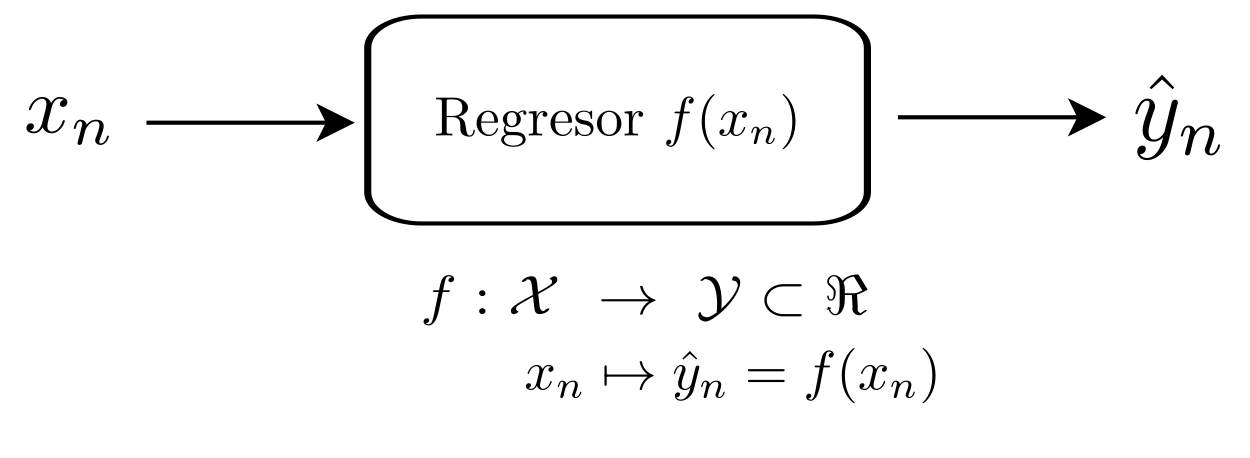
\includegraphics[width=0.9\linewidth]{imgs/def01/task05.png}
            \end{figure}
        \end{itemize}
    \end{frame}

    \begin{frame}{II~$\rhd$~Definición de \textit{Aprendizaje}}
    \framesubtitle{Tipos de \textit{Task} \( T \)}
        \textbf{\Large{\( T \): Regresión Múltiple}}
        \vspace{2mm}
        \begin{itemize}
            \item \textcolor{crimson}{Problema} que busca predecir aquel \textcolor{crimson}{vector} $K$-dimensional de valores \textcolor{crimson}{cuantitativos o continuos en $\Re$} del espacio $\mathcal{Y}\subset\Re^{K}$.
            \vspace{1mm}
            \begin{figure}
                \centering
                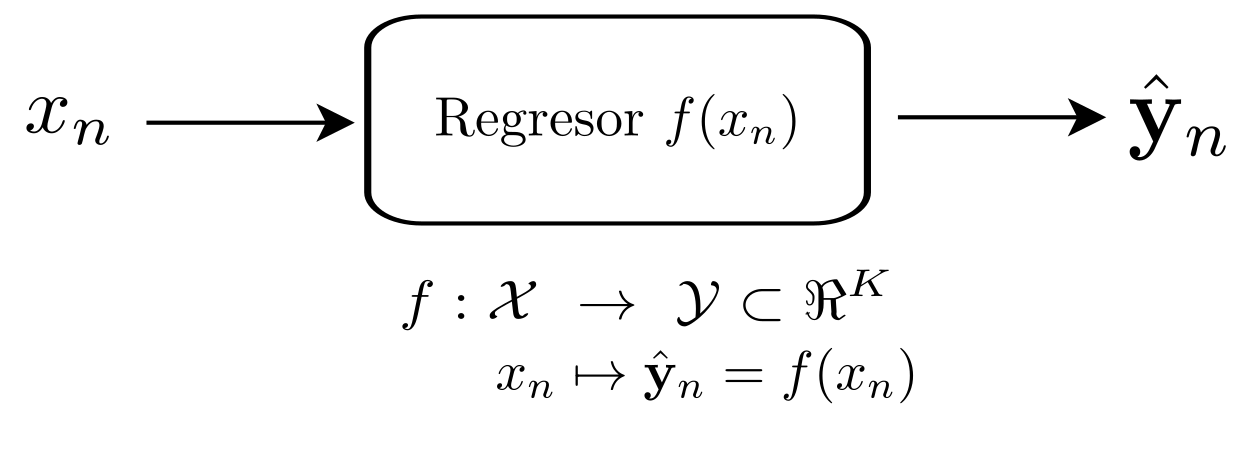
\includegraphics[width=0.9\linewidth]{imgs/def01/task06.png}
            \end{figure}
        \end{itemize}
    \end{frame}

    \begin{frame}{II~$\rhd$~Definición de \textit{Aprendizaje}}
    \framesubtitle{Tipos de \textit{Task} \( T \)}
        \textbf{\Large{\( T \): Regresión Múltiple}}
        \vspace{3mm}
        \begin{itemize}
            \item Una regresión múltiple se puede transformar en $K$ regresiones simples.
            %\pause
            \item Pero! En una regresión múltiple pueden existir una \textit{correlaciones} entre las dimensiones del espacio $\mathcal{Y}$.
        \end{itemize}
    \end{frame}

    \begin{frame}{II~$\rhd$~Definición de \textit{Aprendizaje}}
    \framesubtitle{Tipos de \textit{Task} \( T \)}
        \centering
        \textbf{\Large{¿Pero qué ocurre en el caso cuando $\mathbf{x_{n}}\in\Re^{D}$ con $D>1$?}}\\
        %\pause
        \vspace{15mm}
        \textbf{\Large{$\blacktriangleright$~ Tenemos una tarea de predicción estructurada}}
    \end{frame}

    \begin{frame}{II~$\rhd$~Definición de \textit{Aprendizaje}}
    \framesubtitle{Representación en $\mathcal{X}\subset\Re^{D}$}
        \textbf{\Large{Sobre Espacios Típicos $\mathcal{X}$}}
        \vspace{4mm}
        \begin{itemize}
            \item La mayoría de los métodos predicción van a considerar \textit{Input Values} del tipo $D$-dimensional, tal que $\mathcal{X}\subset\Re^{N\times D}$, y donde cada input será un vector del tipo $\mathbf{x_{n}}\in\Re^{D}$.\footnote{Recuerden que $n=1,2,\cdots,N$, y donde $n$ se refiere a la fila $n$-ésima de un dataframe.}
            %\pause
            \item Cada elemento $D$ del vector $\mathbf{x_{n}}$ será llamado \textbf{feature} o \textbf{característica}.
        \end{itemize}
        \begin{figure}
            \centering
            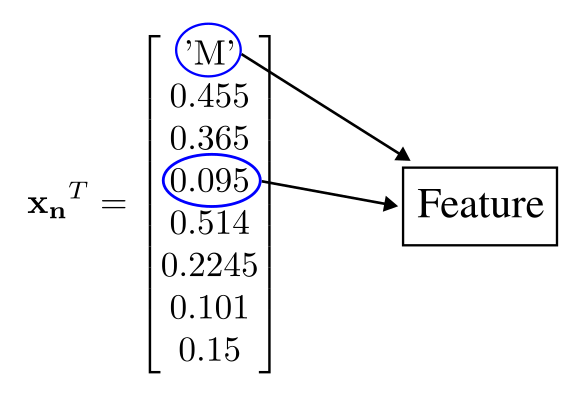
\includegraphics[width=0.45\linewidth]{imgs/def01/taskSpace01.png}
        \end{figure}
    \end{frame}

    \begin{frame}{II~$\rhd$~Definición de \textit{Aprendizaje}}
    \framesubtitle{Representación en $\mathcal{X}\subset\Re^{D}$}
        \textbf{\Large{Representación tipo \textit{DataFrame}}}
        \begin{figure}
            \centering
            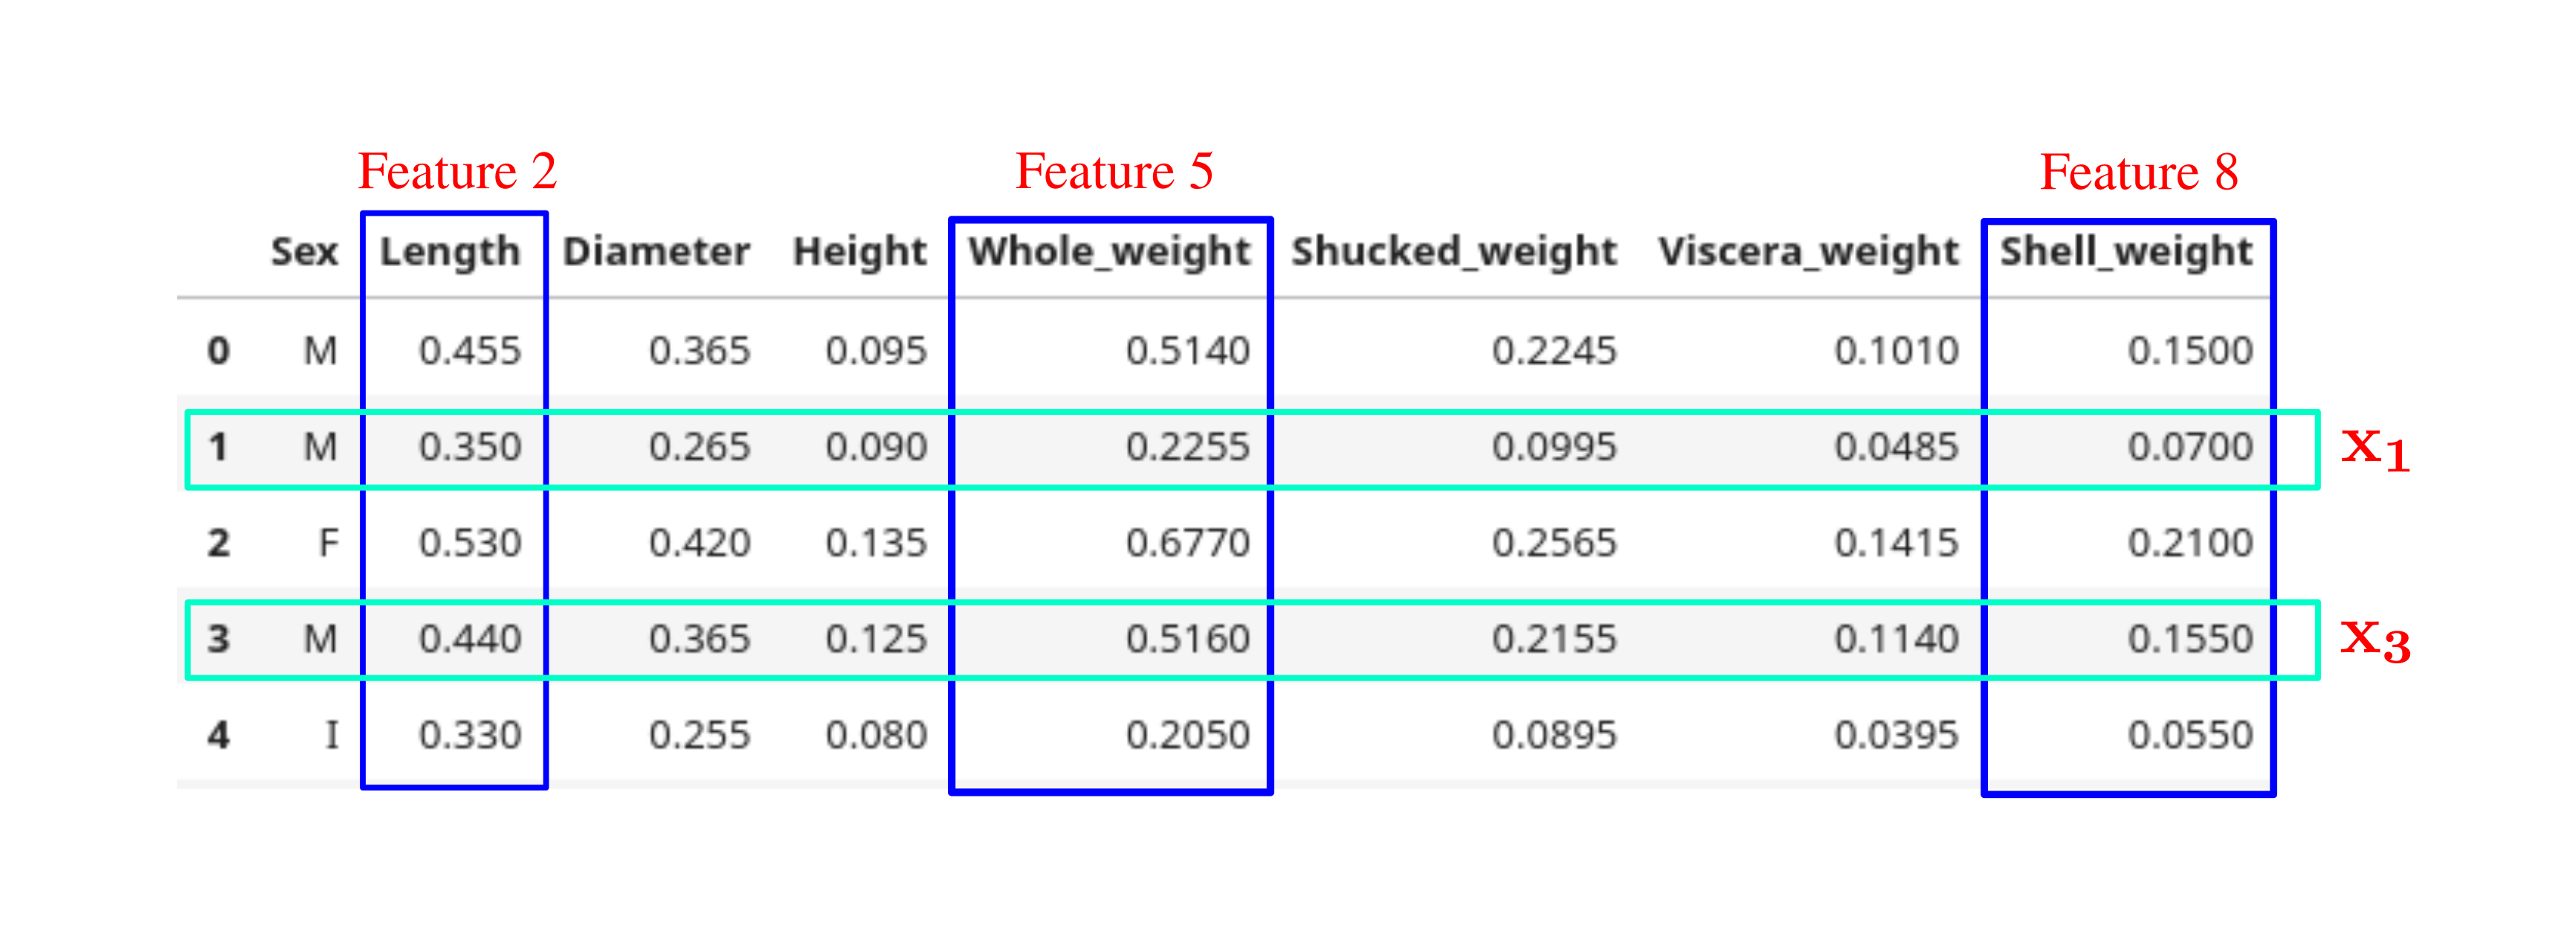
\includegraphics[width=\linewidth]{imgs/def01/taskSpace02.png}
        \end{figure}
        %\pause
        \begin{equation*}
        \scriptsize{
            \mathcal{X}\subset\Re^{5\times 8} = \begin{bmatrix}
            \text{M} & 0.455 & 0.365 & 0.095 & 0.514 & 0.2245 & 0.101 & 0.15 \\
            \text{M} & 0.35 & 0.265 & 0.09 & 0.2255 & 0.0995 & 0.0485 & 0.07 \\
            \text{F} & 0.53 & 0.42 & 0.135 & 0.677 & 0.2565 & 0.1415 & 0.21 \\
            \text{M} & 0.44 & 0.365 & 0.125 & 0.516 & 0.2155 & 0.114 & 0.155 \\
            \text{I} & 0.33 & 0.255 & 0.08 & 0.205 & 0.0895 & 0.0395 & 0.055
            \end{bmatrix}
        }
        \end{equation*}
    \end{frame}

    \begin{frame}{II~$\rhd$~Definición de \textit{Aprendizaje}}
    \framesubtitle{Tipos de \textit{Task} \( T \) Complejas}
        \textbf{\Large{\( T \): Predicación Estructurada}}
        \vspace{2mm}
        \begin{itemize}
            \item \textcolor{crimson}{Problema} que busca predecir un output que NO es un número continuo, una categoría, o un vector; sino un \textcolor{DarkOrchid}{conjunto de valores relacionados} entre ellos.
            \vspace{1mm}
            \begin{figure}
                \centering
                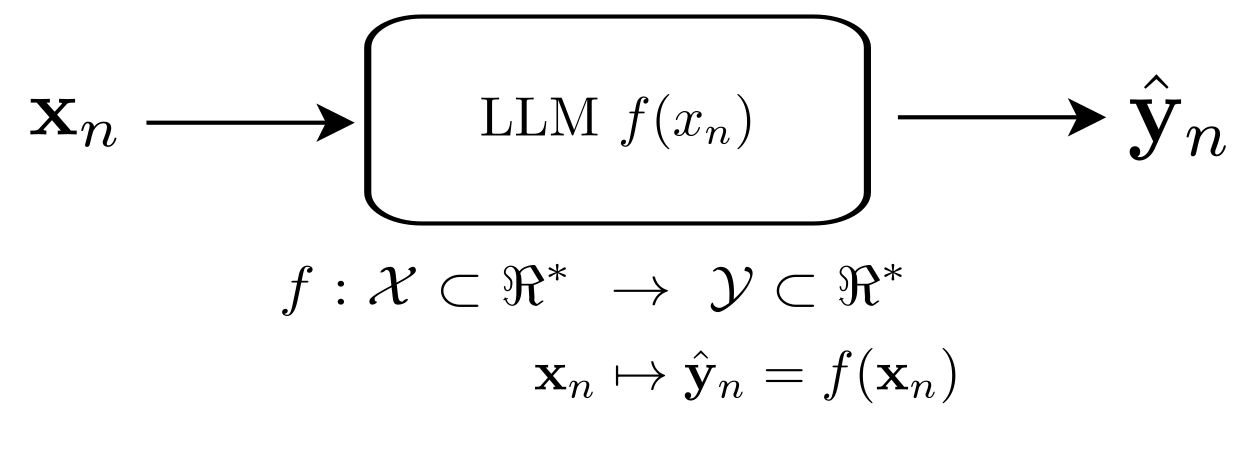
\includegraphics[width=0.8\linewidth]{imgs/def01/task07.png}
            \end{figure}
        \end{itemize}
    \end{frame}

    \begin{frame}{II~$\rhd$~Definición de \textit{Aprendizaje}}
    \framesubtitle{Tipos de \textit{Task} \( T \) Complejas}
        \textbf{\Large{\( T \): Predicación Estructurada}}
        \vspace{2mm}
        \begin{figure}
            \centering
            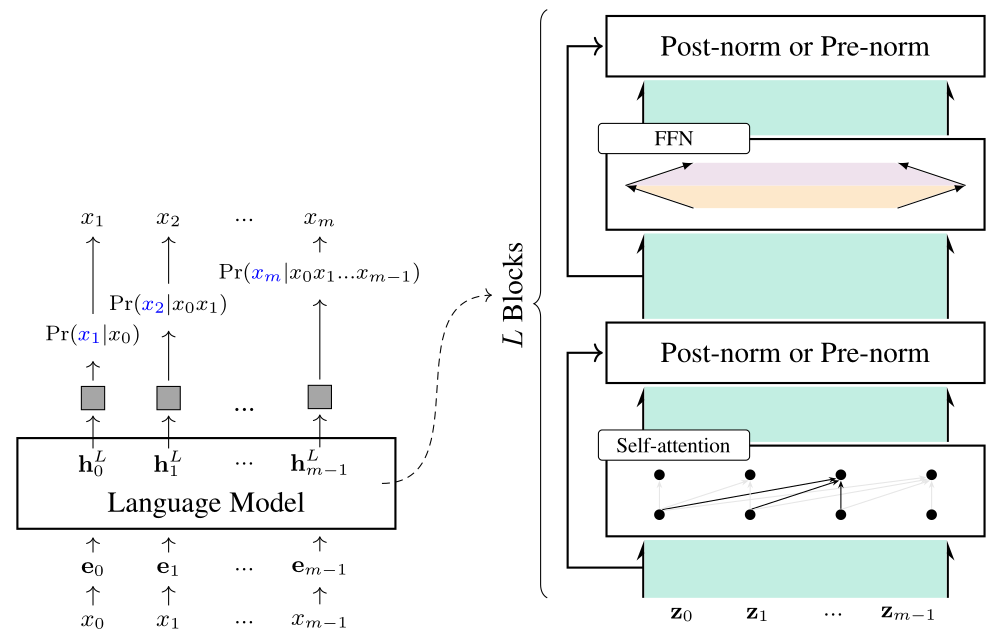
\includegraphics[width=0.7\linewidth]{imgs/def01/xiao2025foundationslargelanguagemodels-img01.png}
            \caption{Arquitectura Transformer-decoder para el procesamientos e lenguaje natural.\footnote{\tiny{Xiao, T., \& Zhu, J. (2025). Foundations of Large Language Models (Version 1). arXiv. \url{https://doi.org/10.48550/ARXIV.2501.09223}}}}
        \end{figure}
    \end{frame}

    \begin{frame}{II~$\rhd$~Definición de \textit{Aprendizaje}}
    \framesubtitle{Tipos de \textit{Task} \( T \) Complejas}
        \textbf{\Large{\( T \): Predicación Estructurada}}
        \vspace{2mm}
        \begin{itemize}
            \item \textcolor{crimson}{Problema} que busca predecir un output que NO es un número continuo, una categoría, o un vector; sino un \textcolor{DarkOrchid}{conjunto de valores relacionados} entre ellos.
            \vspace{1mm}
            \begin{figure}
                \centering
                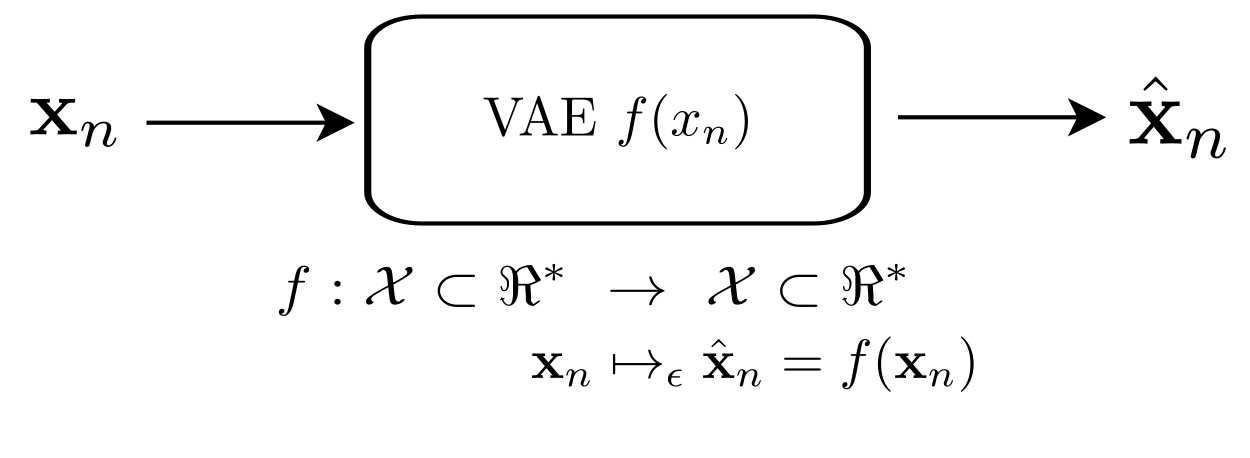
\includegraphics[width=0.8\linewidth]{imgs/def01/task08.png}
            \end{figure}
        \end{itemize}
    \end{frame}

    \begin{frame}{II~$\rhd$~Definición de \textit{Aprendizaje}}
    \framesubtitle{Tipos de \textit{Task} \( T \) Complejas}
        \textbf{\Large{\( T \): Predicación Estructurada}}
        \vspace{2mm}
        \begin{figure}
            \centering
            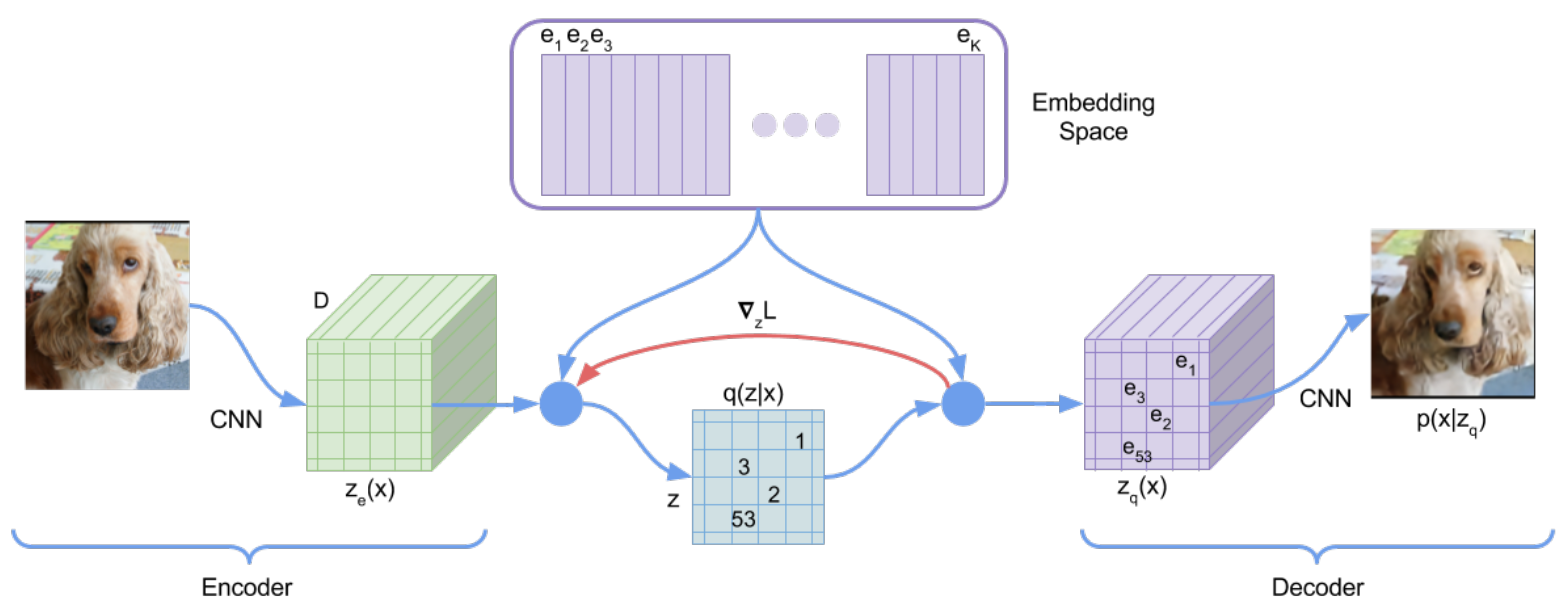
\includegraphics[width=0.9\linewidth]{imgs/def01/oord2018neuraldiscreterepresentationlearning-img01.png}
            \caption{Arquitectura VQ-VAE.\footnote{\tiny{Oord, A. van den, Vinyals, O., \& Kavukcuoglu, K. (2017). Neural Discrete Representation Learning (Version 2). arXiv. \url{https://doi.org/10.48550/ARXIV.1711.00937 }}}}
        \end{figure}
    \end{frame}

    \begin{frame}{II~$\rhd$~Definición de \textit{Aprendizaje}}
    \framesubtitle{Tipos de \textit{Task} \( T \) Complejas}
        \textbf{\Large{\( T \): Predicación Estructurada}}
        \vspace{2mm}
        \begin{itemize}
            \item \textcolor{crimson}{Problema} que busca predecir un output que es una \textcolor{DarkOrchid}{densidad de probabilidad}.
            \vspace{1mm}
            \begin{figure}
                \centering
                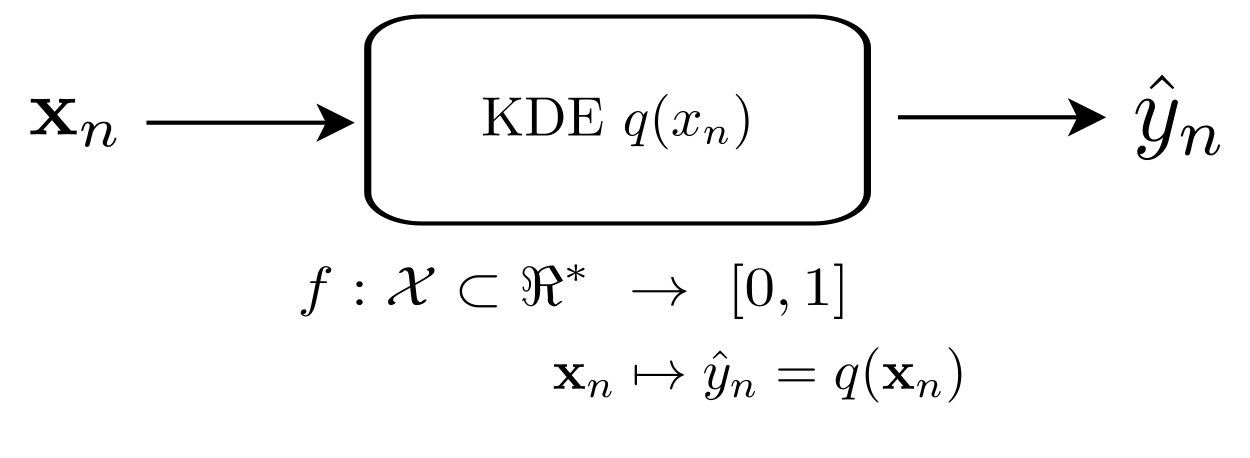
\includegraphics[width=0.9\linewidth]{imgs/def01/task09.png}
            \end{figure}
        \end{itemize}
    \end{frame}

    \begin{frame}{II~$\rhd$~Definición de \textit{Aprendizaje}}
    \framesubtitle{Tipos de \textit{Task} \( T \) Complejas}
        \textbf{\Large{\( T \): Predicación Estructurada}}
        \vspace{2mm}
        \begin{figure}
            \centering
            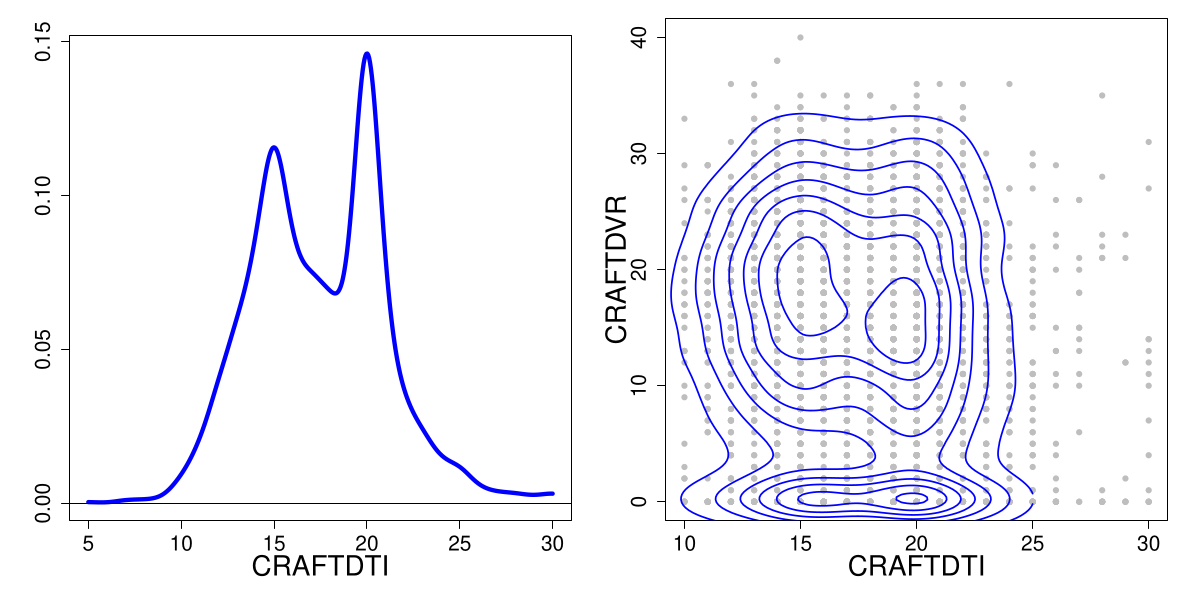
\includegraphics[width=0.7\linewidth]{imgs/def01/chen2017tutorialkerneldensityestimation-img01.png}
            \caption{Ejemplo de la aplicación de KDE sobre el dataset NACC.\footnote{\tiny{Chen, Y.-C. (2017). A Tutorial on Kernel Density Estimation and Recent Advances (Version 2). arXiv. \url{https://doi.org/10.48550/ARXIV.1704.03924 }}}}
        \end{figure}
    \end{frame}

    \section{Definición Training Experience \( E \)}
    \begin{frame}{III~$\rhd$~Definición de \textit{Aprendizaje}}
    \framesubtitle{Definición Training Experience \( E \)}
        \begin{block}{Definición Training Experience \( E \)}
        Es aquella \textbf{información} que se le proporciona al programa durante la fase de \textbf{entrenamiento}, en orden de optimizar la solución al \textbf{problema}.
        \end{block}
        %\pause
        \vspace{5mm}
        \begin{itemize}
            \item La información entregada corresponde al conjunto de datos que representan ejemplos de una solución esperada al problema.
            %\pause
            \item Lo llamaremos dataset de entrenamiento o training set $S$.
        \end{itemize}
    \end{frame}
    
    \begin{frame}{III~$\rhd$~Definición de \textit{Aprendizaje}}
    \framesubtitle{Tipos Training Experience \( E \)}
        \begin{block}{Aprendizaje Supervisado}\footnote{\textcolor{DarkOrchid}{En futuras definiciones, vamos a asumir por defecto siempre que se trata de un entrenamiento supervenido, a menos que se diga lo contrario.}}
        Se dispone de un conjunto de $N$ inputs con el respectivo valor de la solución al problema.
        %\pause
        \begin{equation*}
            \mathcal{S}=\left\{\mathbf{x_{n}},~y_{n}\right\}^{N}_{n=0}\coloneq \left\{ \left(\mathbf{x_{0}},~y_{0}\right), \left(\mathbf{x_{1}},~y_{1}\right), \cdots, \left(\mathbf{x_{N}},~y_{N}\right) \right\},
        \end{equation*}
        donde $\mathbf{x_{n}}\in\Re^{D}$, $D\geq1$, e $y_{n}\in\Re$.\\
        %\pause
        \vspace{2mm}
        $\rhd$~Supuestos típico para las tareas de regresión y clasificación.\\
        %\pause
        $\rhd$~\textcolor{DarkOrchid}{Es importante que $\left\{\mathbf{x_{n}},~y_{n}\right\}\sim\text{idd}$}.
        \end{block}
    \end{frame}

    \begin{frame}{III~$\rhd$~Definición de \textit{Aprendizaje}}
    \framesubtitle{Tipos Training Experience \( E \)}
        \textbf{\Large{Aprendizaje Supervisado}}
        \vspace{2mm}
        \begin{figure}
            \centering
            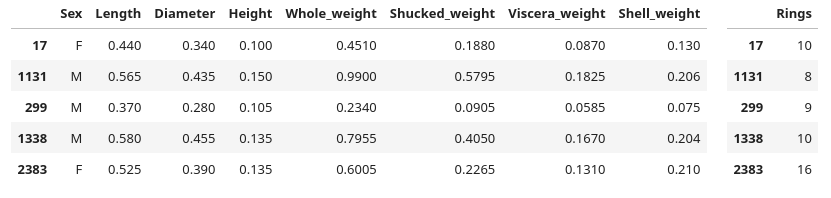
\includegraphics[width=0.7\linewidth]{imgs/def02/abalone-df.png}
            \caption{Abalone Dataset. Predecir la \textbf{edad} de los abalones a partir de características físicas. 1995.}
        \end{figure}
        \begin{figure}
            \centering
            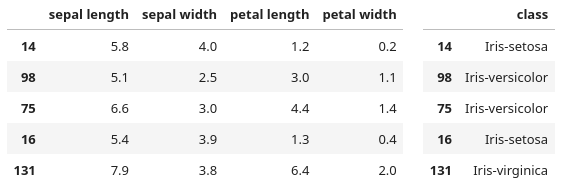
\includegraphics[width=0.55\linewidth]{imgs/def02/iris-df.png}
            \caption{Iris Dataset. Predecir la \textbf{clase} de las plantas Iris a partir de características físicas. Ronald Fisher 1936.}
        \end{figure}
    \end{frame}

    \begin{frame}{III~$\rhd$~Definición de \textit{Aprendizaje}}
    \framesubtitle{Tipos Training Experience \( E \)}
        \begin{block}{Aprendizaje No Supervisado}
        Se dispone de un conjunto de $N$ inputs SIN el respectivo valor de la solución al problema.
        %\pause
        \begin{equation*}
            \mathcal{S}=\left\{\mathbf{x_{n}}\right\}^{N}_{n=0}\coloneq \left\{ \left(\mathbf{x_{0}}\right), \left(\mathbf{x_{1}}\right), \cdots, \left(\mathbf{x_{N}}\right) \right\},
        \end{equation*}
        donde $\mathbf{x_{n}}\in\Re^{D}$, $D\geq1$.\\
        %\pause
        \vspace{2mm}
        $\rhd$~Supuestos típico paras las tareas de detección de anomalías, reconstrucción de imágenes, y estimación de densidades de probabilidad.
        \end{block}
    \end{frame}

    \section{Sobre la \textit{Hipotiposis}}
    \begin{frame}{IV~$\rhd$~Definición de \textit{Aprendizaje}}
    \framesubtitle{Sobre la \textit{Hipotiposis}}
        \begin{itemize}
            \item Para aproximar la función desconocida, nuestra máquina debe observar casos del tipo input-output.
            %\pause
            \item Dado un input, la maquinas tratara de predecir el output más correcto.
            \begin{figure}
                \centering
                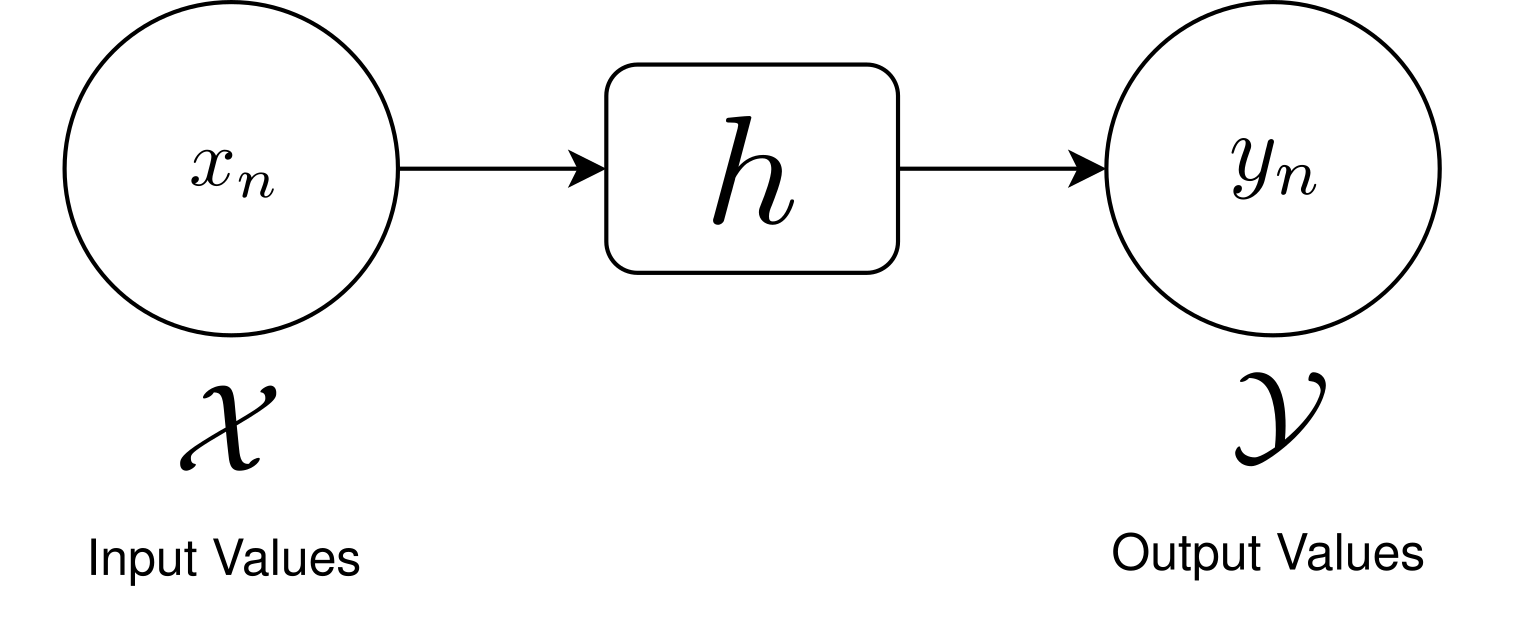
\includegraphics[width=0.8\linewidth]{imgs/def02/exp01.png}
            \end{figure}
            %\pause
            \item La función que busca nuestra máquina será la \textbf{\textcolor{crimson}{hipotiposis}}.
        \end{itemize}  
    \end{frame}

    \begin{frame}{IV~$\rhd$~Definición de \textit{Aprendizaje}}
    \framesubtitle{Sobre la \textit{Hipotiposis}}
        \begin{figure}
            \centering
            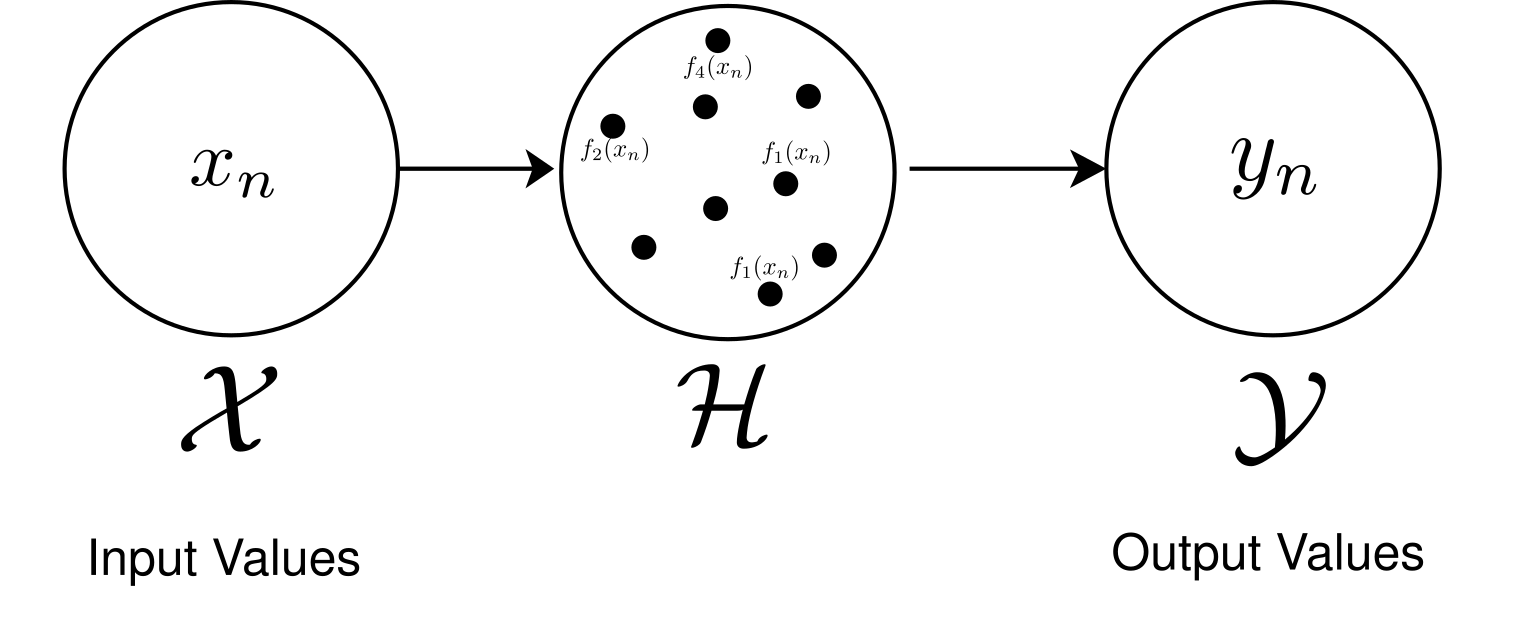
\includegraphics[width=\linewidth]{imgs/def02/exp02.png}
        \end{figure}
    \end{frame}

    \begin{frame}{IV~$\rhd$~Definición de \textit{Aprendizaje}}
    \framesubtitle{Espacio de \textit{Hipotiposis}}
        \begin{block}{Espacio $\mathcal{H}$}
        Conjunto de todas las \textbf{posibles soluciones} dadas por las \textbf{funciones} que la máquina puede implementar para el problema dado.
        \end{block}
        \begin{figure}
            \centering
            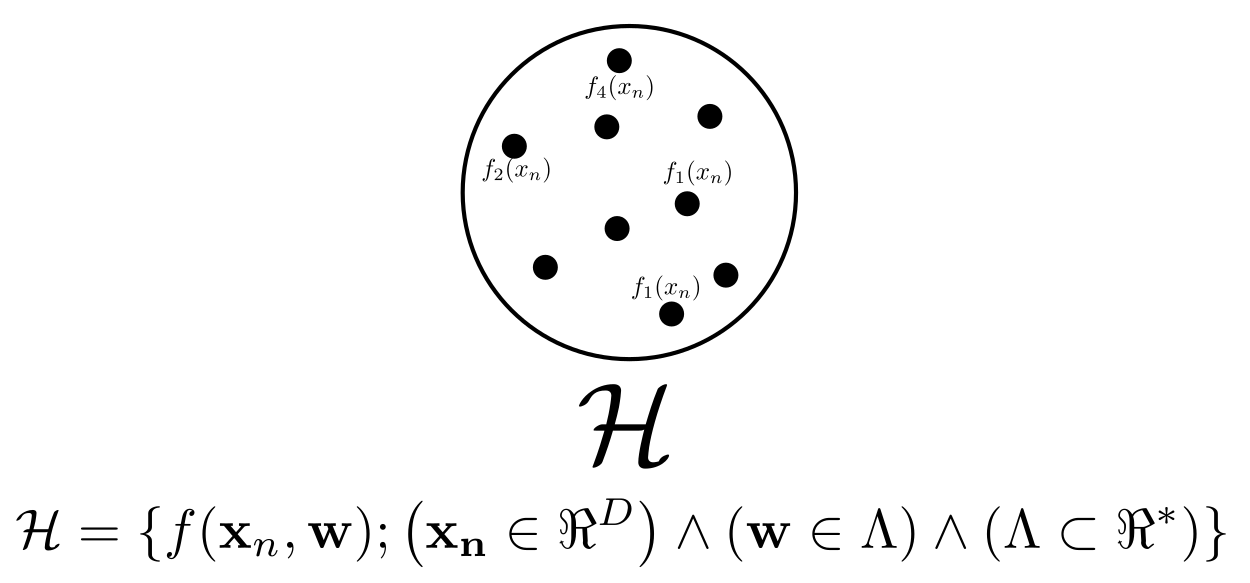
\includegraphics[width=0.8\linewidth]{imgs/def03/measure01.png}
        \end{figure}
    \end{frame}

    \begin{frame}{IV~$\rhd$~Definición de \textit{Aprendizaje}}
    \framesubtitle{Espacio de \textit{Hipotiposis}}
        \begin{figure}
            \centering
            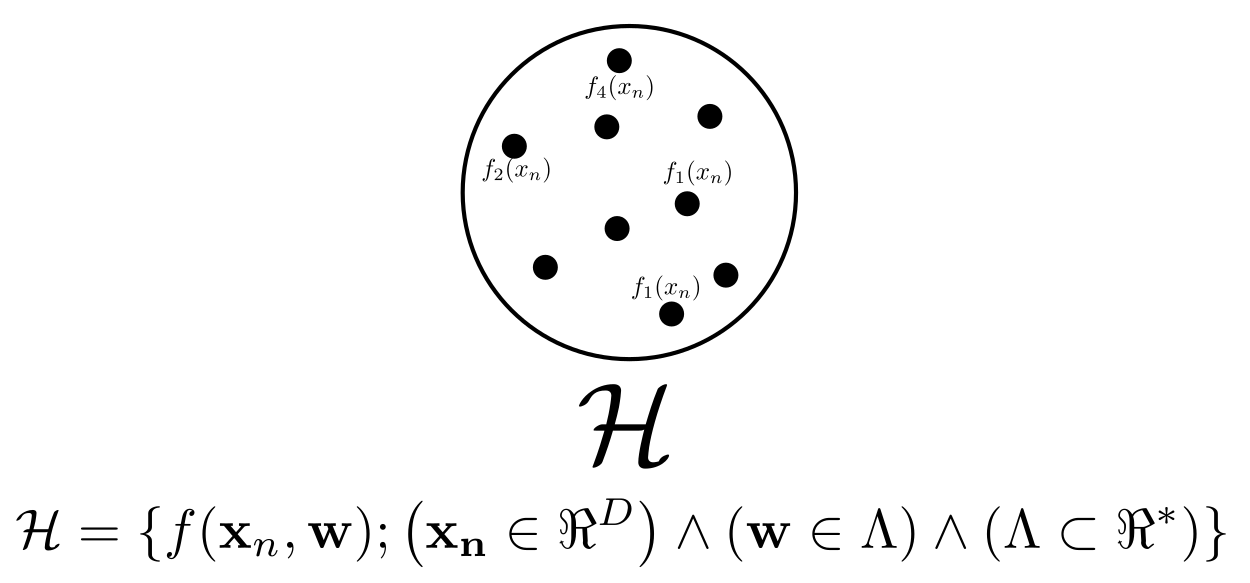
\includegraphics[width=0.55\linewidth]{imgs/def03/measure01.png}
        \end{figure}
        \begin{itemize}
            \item El espacio $\mathcal{H}$ esta \textbf{parametrizado}, y por lo tanto, cada función $f(\mathbf{x}_{n}, \mathbf{w})$ queda identificada por un conjunto finito de parámetros $\mathbf{w}$.
            %\pause
            \item De este modo, vamos a definir $\mathbf{w}$ como los \textbf{parámetros del modelo} y conjunto $\Lambda$ como el espacio de parámetros.
            %\pause
            \item En la práctica, la máquina no va trabajar sobre función $f(*)$, sino sobre el espacio de parámetros $\Lambda$.
        \end{itemize}
    \end{frame}

    \section{Definición Performance Measure \( P \)}
    \begin{frame}{V~$\rhd$~Definición de \textit{Aprendizaje}}
    \framesubtitle{Definición Performance Measure \( P \)}
        \begin{block}{Definición Performance Measure \( P \)}
        Es aquella función $R$ sobre el espacio de hipótesis $\mathcal{H}$ que permite \textbf{medir cuantitativamente} la \textbf{calidad} de la función $f(\mathbf{x}_{n}, \mathbf{w})$, implementada por la máquina.
        \end{block}
        \vspace{3mm}
        \begin{figure}
            \centering
            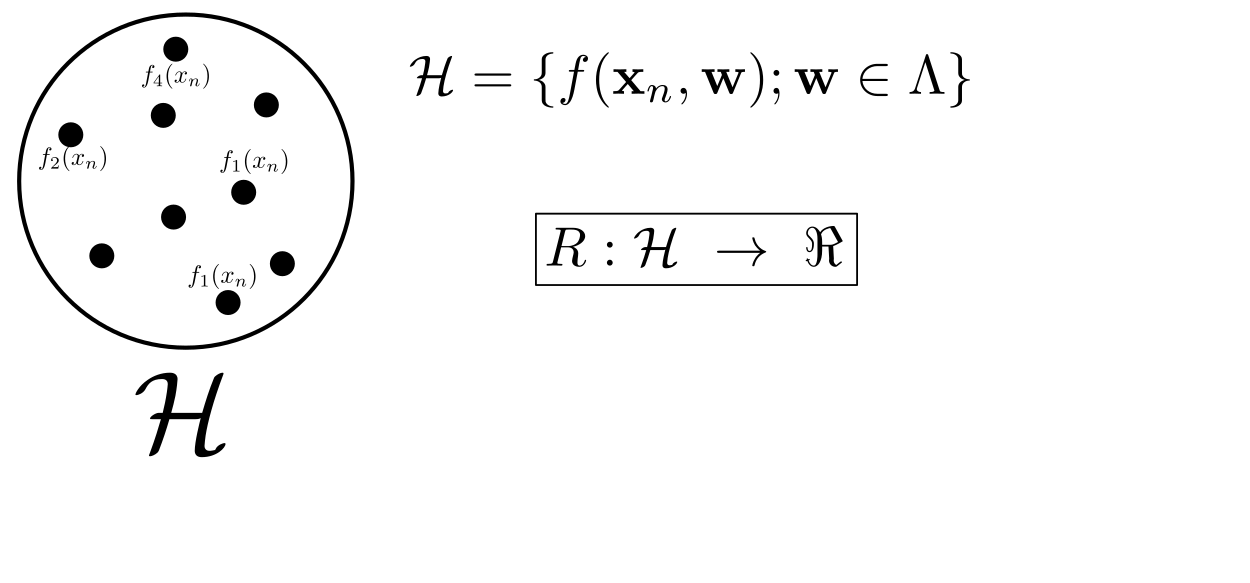
\includegraphics[width=0.8\linewidth]{imgs/def03/measure02.png}
        \end{figure}
    \end{frame}

    \begin{frame}{V~$\rhd$~Definición de \textit{Aprendizaje}}
    \framesubtitle{Definición Performance Measure \( P \)}
        \begin{block}{Definición Función de Perdida $\ell$}
        La funcion $\ell$ permite medir cuantitativamente la calidad de la hipótesis dada por $\hat{y}=f(x_{n})$, la cual implementa la maquina para un correspondiente input $x_{n}$ y su posible respuesta $\hat{y}$ 
        \end{block}
        \vspace{3mm}
        \begin{figure}
            \centering
            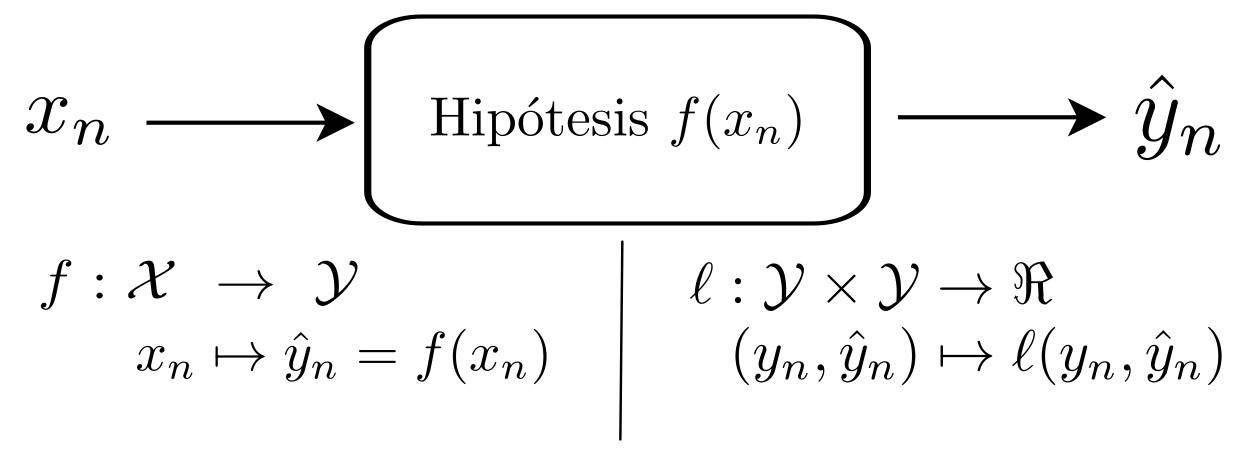
\includegraphics[width=0.8\linewidth]{imgs/def03/measure03.png}
        \end{figure}
    \end{frame}

    \begin{frame}{V~$\rhd$~Definición de \textit{Aprendizaje}}
    \framesubtitle{Definición Performance Measure \( P \)}
        \textbf{\Large{Definición Función de Perdida $\ell$}}
        \begin{figure}
            \centering
            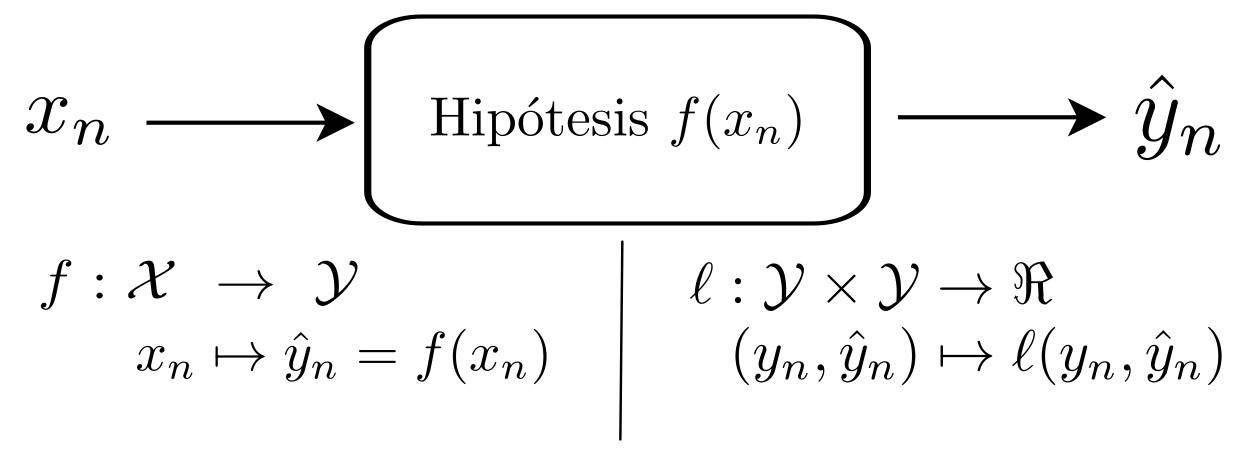
\includegraphics[width=0.5\linewidth]{imgs/def03/measure03.png}
        \end{figure}
        \begin{itemize}
            \item La función $\ell$ suele ser conocida como: \textit{loss function}.
            %\pause
            \item La etiqueta $y$ suele ser llamada \textit{ground truth}.
            %\pause
            \item Por lo general ocurre que $\ell:\mathcal{Y}\times\mathcal{Y}\rightarrow\Re^{+}_{0}$.
            %\pause
            \item $>\ell$ equivale a menor desempeño, mientra que $<\ell$ equivale a un mejor desempeño.
        \end{itemize}
    \end{frame}

    \begin{frame}{V~$\rhd$~Definición de \textit{Aprendizaje}}
    \framesubtitle{Ejemplos de Funciones de Perdida $\ell$}
        \textbf{\Large{Task: Clasificación}}
        \begin{figure}
            \centering
            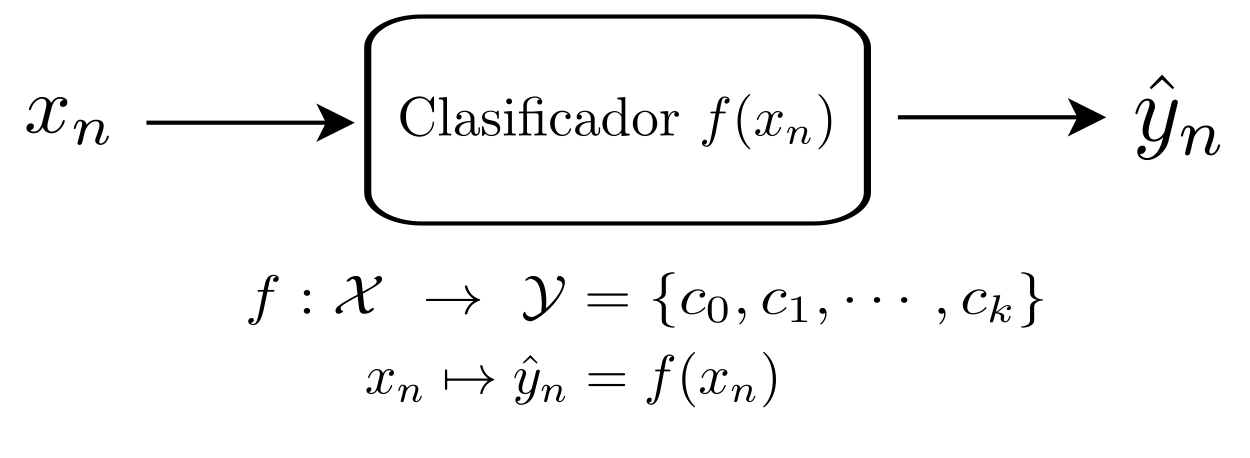
\includegraphics[width=0.7\linewidth]{imgs/def01/task03.png}
        \end{figure}
        \textbf{\Large{Misclassification Loss}\footnote{Donde $\mathbb{I}(*)$ es la función indicatriz.}}
        \begin{equation*}
            \ell(y, \hat{y}) = \mathbb{I}(y \neq \hat{y}) = 
            \begin{cases} 
            0 & \text{si } y = \hat{y}, \\
            1 & \text{si } y \neq \hat{y}.
            \end{cases}
        \end{equation*}
    \end{frame}

    \begin{frame}{V~$\rhd$~Definición de \textit{Aprendizaje}}
    \framesubtitle{Ejemplos de Funciones de Perdida $\ell$}
        \textbf{\Large{Task: Regresión}}
        \begin{figure}
            \centering
            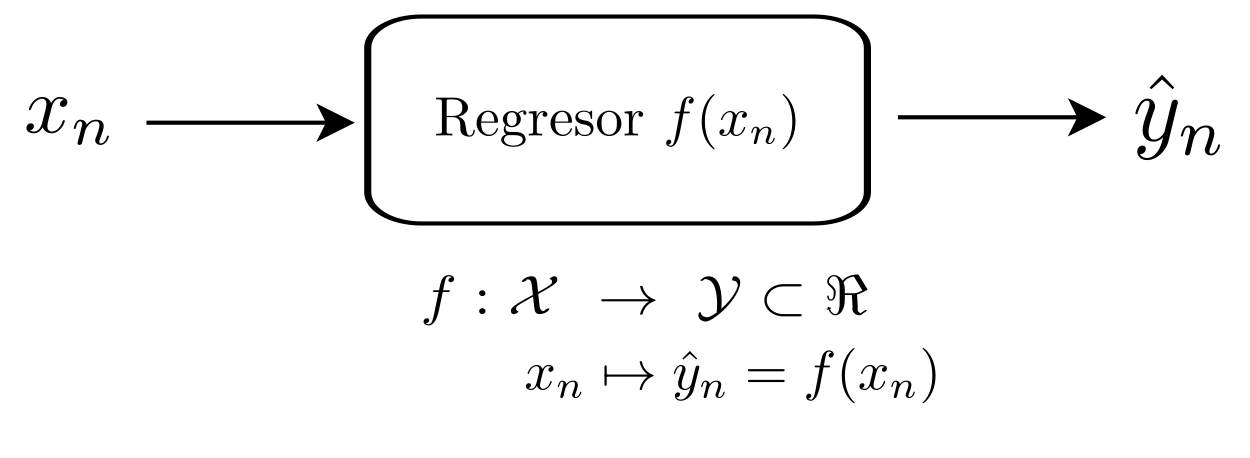
\includegraphics[width=0.6\linewidth]{imgs/def01/task05.png}
        \end{figure}
        \textbf{\Large{Squered Loss}}
        \begin{equation*}
            \ell(y, \hat{y}) = (y-\hat{y})^{2}
        \end{equation*}
        \textbf{\Large{Epsilon Insensitive Loss}}
        \begin{equation*}
            \ell(y, \hat{y}) = 
            \begin{cases} 
            \hfill 0 \hfill & \text{si } |y - \hat{y}| \leq \epsilon, \\[5pt]  
            \hfill |y - \hat{y}| - \epsilon \hfill & \text{etoc}.
            \end{cases}
        \end{equation*}
    \end{frame}

    \begin{frame}{V~$\rhd$~Definición de \textit{Aprendizaje}}
    \framesubtitle{Definición Performance Measure \( P \)}
        \begin{block}{Definición Performance Measure \( P \)}
        Es aquella función $R$ sobre el espacio de hipótesis $\mathcal{H}$ que permite \textbf{medir cuantitativamente} la \textbf{calidad} de la función $f(\mathbf{x}_{n}, \mathbf{w})$, implementada por la máquina.\\
        %\pause
        \vspace{2mm}
        $\rhd$~\textcolor{DarkOrchid}{Dado los $N$ valores de la evaluación $\ell(y_{n},\hat{y}_{n})$, con $n=0,1,\cdots,N$, el desempeño global de la máquina viene dado por la función de agregación $R$.}
        \end{block}
        \begin{figure}
            \centering
            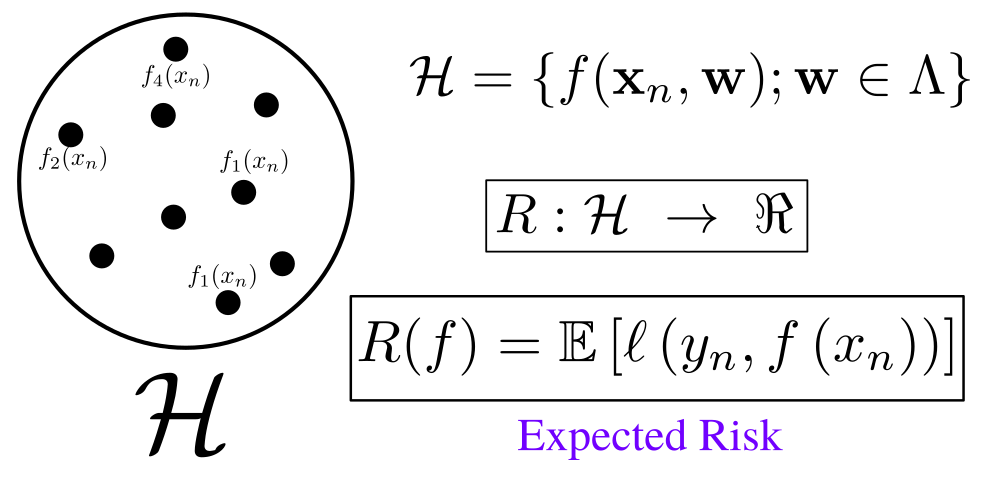
\includegraphics[width=0.5\linewidth]{imgs/def03/measure04.png}
        \end{figure}
        %\pause
        \textit{Cual es el valor $\mathbb{E}$ de un conjunto iid ?}%\pause~$\Rightarrow$~la media 
    \end{frame}

    \begin{frame}{V~$\rhd$~Definición de \textit{Aprendizaje}}
    \framesubtitle{Definición Performance Measure \( P \)}
        \textit{Cual es el valor $\mathbb{E}$ de un conjunto iid ?}~$\Rightarrow$~la media
        \begin{figure}
            \centering
            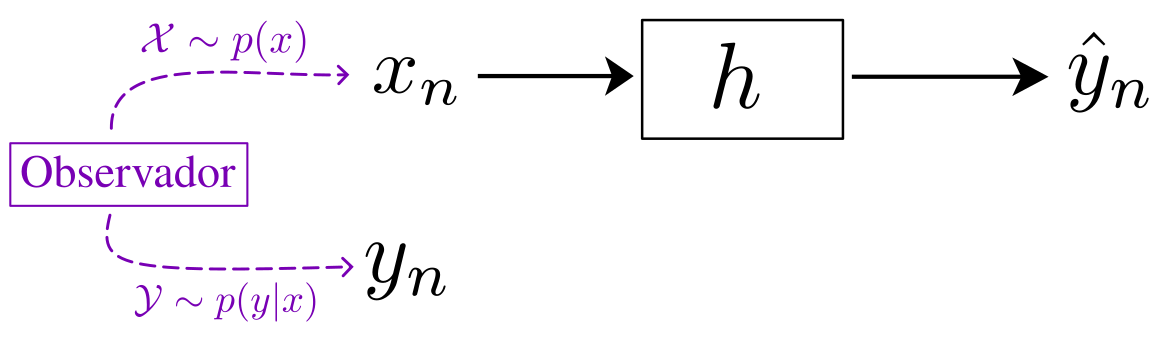
\includegraphics[width=0.8\linewidth]{imgs/def03/measure05.png}
        \end{figure}
        \vspace{3mm}
        %\pause
        \begin{equation*}
            \mathbb{E}_{\mathcal{X},\mathcal{Y}}\left[\ell\left(y,~f\left(x\right)\right)\right] = \int_{\mathcal{X},\mathcal{Y}}{\ell\left(y,~f\left(x\right)\right)\cdot p\left(y,~f\left(x\right)\right)}\,dx\,dy
        \end{equation*}
        \vspace{3mm}
        %\pause
        \begin{equation*}
            \mathbb{E}_{\mathcal{X},\mathcal{Y}}\left[\ell\left(y,~f\left(x\right)\right)\right] = \sum_{x\in\mathcal{X},y\in\mathcal{Y}}{\ell\left(y,~f\left(x\right)\right)\cdot p\left(y,~f\left(x\right)\right)}
        \end{equation*}
    \end{frame}

    \begin{frame}{V~$\rhd$~Objetivo del Aprendizaje}
        \begin{block}{Minimización del \textbf{Expected Risk}}
            Buscamos una función $f(*)$ tal que minimice el \textbf{Expected Risk} $\mathbb{E}$.
            \begin{equation*}
                \min R(f)=\mathbb{E}\left[\ell\left(y,f\left(x\right)\right)\right]\text{ sujeto a } f\in\mathcal{H}
            \end{equation*}
        \end{block}
        \begin{figure}
            \centering
            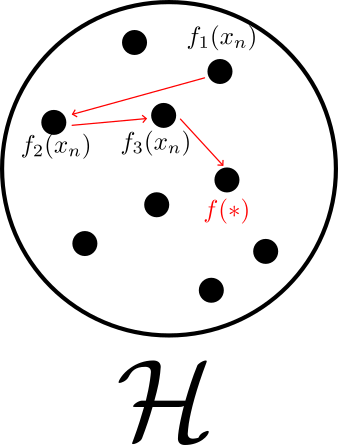
\includegraphics[width=0.25\linewidth]{imgs/def03/measure06.png}
        \end{figure}
    \end{frame}

    \begin{frame}{V~$\rhd$~Objetivo del Aprendizaje}
        \begin{block}{Minimización del \textbf{Expected Risk}}
            Buscamos el vector de paramentos $\mathbf{w}^{*}$ para la función $f(x, \mathbf{w}^{*})$ tal que minimice el \textbf{Expected Risk} $\mathbb{E}$.
            %\pause
            \begin{equation*}
                \min R(\mathbf{w})=\mathbb{E}\left[\ell\left(y,f\left(x, \mathbf{w}\right)\right)\right]\text{ sujeto a } \mathbf{w}\in\Lambda
            \end{equation*}
        \end{block}
        \begin{figure}
            \centering
            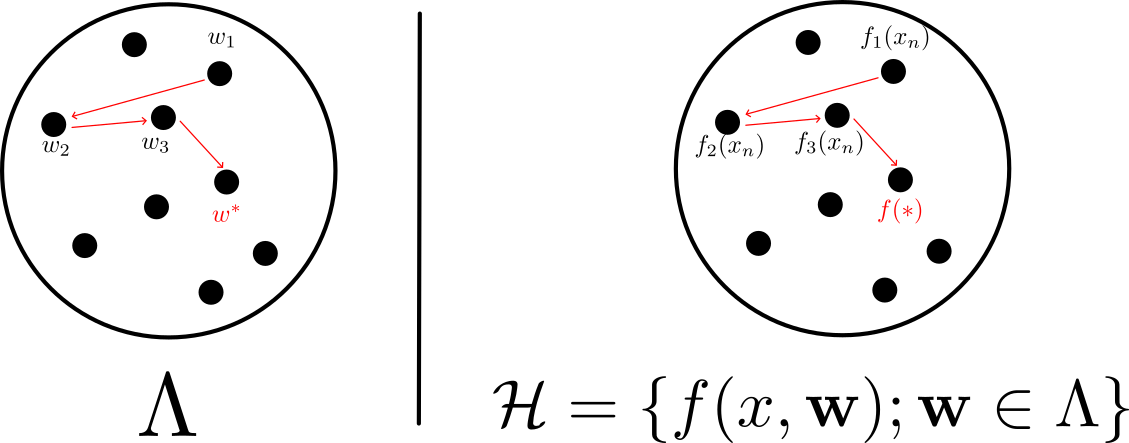
\includegraphics[width=0.85\linewidth]{imgs/def03/measure07.png}
        \end{figure}
    \end{frame}

\end{document}